\documentclass[10pt]{article}
\usepackage[utf8]{inputenc}
\usepackage[T1]{fontenc}
\usepackage{amsmath}
\usepackage{amsfonts}
\usepackage{amssymb}
\usepackage[version=4]{mhchem}
\usepackage{stmaryrd}
\usepackage{graphicx}
\usepackage[export]{adjustbox}
\graphicspath{ {./images/} }
\usepackage{multirow}

\title{Creating a Havannah Playing Agent }


\author{B. Joosten}
\date{}


\begin{document}
\maketitle
August 27, 2009

\begin{abstract}
This paper delves into the complexities of Havannah, which is a 2 -person zero-sum perfectinformation board game. After determining these complexities an appropriate technique for creating a Havannah agent is introduced viz. Monte-Carlo Tree Search (MCTS). The Nearest Neighbour preference enhancement to the MCTS' simulation strategy does not lead to a major increase of performance. The MCTS agent does however have a $76 \%$ win rate against a greedy Monte-Carlo based player.
\end{abstract}

Keywords: Havannah, Monte-Carlo Tree Search, Upper Confidence bound applied to Trees

\section*{1 Introduction}
Havannah is a 2-person, zero-sum, perfect-information, converging, sudden-death, connection game as explained in [1], which has recently drawn the attention of researchers in the field of AI [11]. Havannah was invented by Christian Freeling in 1976 [6] and is played on a board with 271 cells. It has some similarities with the game of Hex. Although Havannah has other goals and a differently shaped board the idea of virtual connections in Hex [10] is quite relevant to Havannah [4, 5]. One of the interesting aspects of the game is that humans are quite capable of quickly understanding the game and its goals. The deceivingly simple goals are extremely hard to program in a computer agent capable of playing Havannah autonomously. The inventor Christian Freeling thinks it is so hard he has even put out a challenge. Anyone who is able to write a Havannah program by 2012 that is capable of beating him once out of ten games will receive $€ 1000$. It is not the winning connections which pose a difficulty to represent but the strategic and tactical objectives to achieve these connections. The way humans are capable of evaluating the course of the game is fascinating and holds the key to solving the game. What is difficult in building a Havannah agent is the lacking of certain game aspects. For instance:

\begin{itemize}
  \item the game has no material imbalance
  \item there is no general direction
\end{itemize}

The absence of these aspects makes it harder to derive heuristics for an agent. This also poses a challenge in examining the capabilities of present AI algorithms used in other 2-person zero-sum perfect-information games.

Giving the high complexity of Havannah, which will be discussed in Section 3, the experiments in this paper have all been conducted on a board with 61 cells. The goal is to create a Havannah game-playing agent. Therefore the following problem statement is formulated:

Which algorithms and heuristics are valuable for the construction of a Havannah game-playing agent?

This leads to the following three research questions which will be answered in this paper:

\begin{itemize}
  \item What is Havannah's state-space complexity and game-tree complexity?
  \item Taking these complexities into account, which algorithms are the most promising to develop a computer agent that is capable of playing Havannah?
  \item Which adjustments and extensions of these algorithms make the agent more advanced?\\
This paper is organized as follows. Section 2 will explain the game of Havannah in more detail. Section 3 will elucidate the concepts of state-space complexity and game-tree complexity by applying them to Havannah. The architecture and a description of the Monte-Carlo Tree Search algorithm are discussed in Section 4. Section 5 will present the results of the experiments conducted. Conclusions and future research are outlined in Section 6 .
\end{itemize}

\section*{2 The Game of Havannah}
Havannah is usually played on a hexagonal board that consists of 271 hexagonal cells. This is called a $19 \times 19$ board. The board allows for a maximum of six directions to expand a connection. The goal of the game is to construct a winning connection before the opponent does. There are three winning connections, viz. the bridge, the fork and the ring. Figure 1 shows these connections on a $9 \times 9$ board. A bridge is a connection between any two corners of the board. A fork is a connection between any three different sides. This connection may not contain

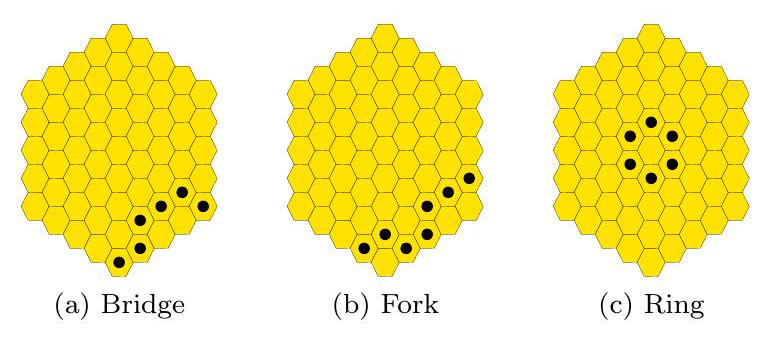
\includegraphics[max width=\textwidth, center]{2024_09_21_575efd6e0a8f951a52dfg-2}\\
Figure 1: End positions\\
corner cells which are indispensable for this connection. A ring is a circular connection enclosing at least one cell, occupied or not. The minimum length of a ring therefore is six. When a player reaches one of these connections the game is won. A draw is theoretically possible, when the complete board is occupied by white and black stones and no winning connection is reached.

A property of hexagonal boards is the possibility of creating virtual connections. Consider the stones in Figure 2. There is no real connection between any of the stones, yet White will not be able to prevent Black from connecting them. These stones are virtually connected by a so called 2-bridge. The stones in Figures 2a and 2 b are not only virtually connected, but they also constitute a virtual winning connection. Such a connection is called a frame. A frame is the most important strategic concept in Havannah [4]. The speed of a frame is the number of stones necessary to complete the winning connection. An opponent's frame can only be parried by a faster frame. Attempts to obstruct the frame lead to a certain loss. The ring threats in Figure 3a are not

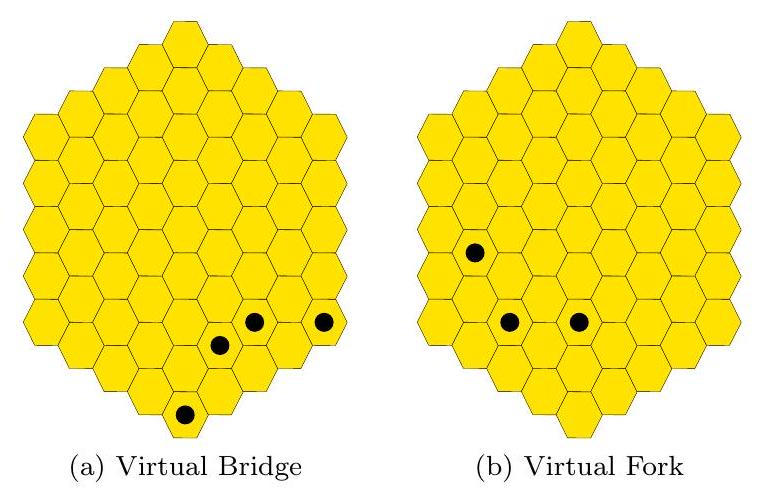
\includegraphics[max width=\textwidth, center]{2024_09_21_575efd6e0a8f951a52dfg-2(1)}\\
Figure 2: Frames\\
frames. The upper threat can be eliminated from the inside while the lower threat can be canceled from the outside as is shown in Figure 3b. While a fork frame can be created using less than half the stones required for the fastest fork, a ring frame needs more than the minimum stone length of a ring.

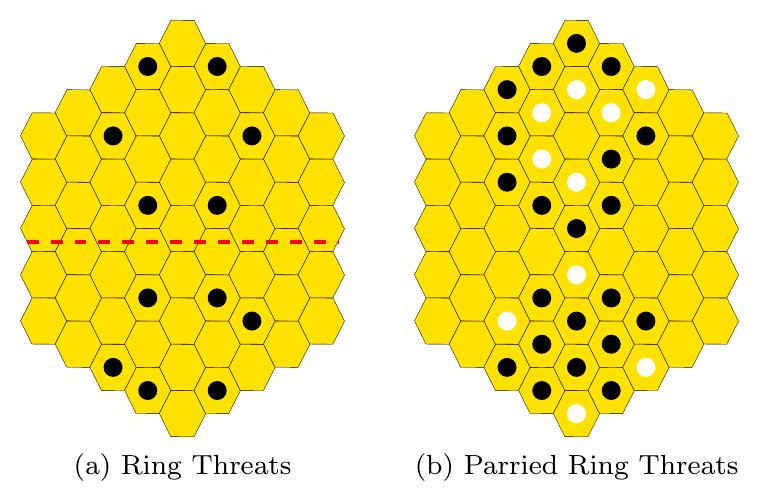
\includegraphics[max width=\textwidth, center]{2024_09_21_575efd6e0a8f951a52dfg-2(2)}\\
Figure 3: Parriable Ring Threats

\section*{3 Havannah's Complexities}
An important property which distinguishes classic board games is complexity [1]. This property implicates two measures, viz. state-space complexity and game-tree complexity. These measures are relevant to give an indication of the approach and computational strain necessary to solve the game. Subsections 3.1 and 3.2 will deal with state-space complexity and game-tree complexity, respectively. First an understanding of the concept is created and then its value for Havannah is determined.

\subsection*{3.1 State-Space Complexity}
State-space complexity is a measure for all different legal states a game can have. For most classic board games this state-space is usually too large for a computer to enumerate all positions. This means a brute-force approach to solve these games is inapplicable. Therefore a broad understanding of the underlying mathematical structures and complex strategies is necessary to narrow the search for a good move, like is done for chess [9]. For most games calculating an exact state-space complexity is infeasible, therefore approximations are used. Starting with a rough estimated upper bound they are refined until a satisfactory upper bound is found.

To create an upper bound to Havannah's state-space complexity a few observations have to be made. Havannah is a game with no movement or capture. This means we can derive an upper bound by summing all the possible combinations for every number of stones. See Formulas 1 and 2.


\begin{equation*}
\sum_{i=1}^{271} N u m\left(\frac{i+i \bmod 2}{2}, \frac{i-i \bmod 2}{2}\right) \tag{1}
\end{equation*}


where


\begin{equation*}
\operatorname{Num}(w, b)=\binom{271}{w} \times\binom{ 271-w}{b} \tag{2}
\end{equation*}


In this formula $w$ and $b$ stand for white and black stones, respectively, in the $i$-th move. For Havannah this means\\
a state-space complexity of $10^{128}$. This upper bound can be improved by observing that Havannah is played on a hexagonal board. Therefore there are six mirror positions possible and six transformations which are symmetrical identical. Through dividing by twelve the statespace complexity is refined to $10^{127}$. This is still a rough estimation, because it does not take into account positions with multiple winning connections.

\subsection*{3.2 Game-Tree Complexity}
The game-tree complexity is an estimate of the size of the minimax search tree which has to be built to solve the game [1]. To explain game-tree complexity two auxiliary definitions have to be introduced.\\
Definition 1. The solution depth of a node $J$ is the minimal depth (in ply) of a full-width search sufficient to determine the game-theoretic value of $J$.

This is the number of plies in which the game will be decided in optimal play. Where a ply is one move of an opponent. In contrast to a turn, which represents two plies.\\
Definition 2. The solution search tree of a node $J$ is the full-width search tree with a depth equal to the solution depth of $J$.

Combining these two definitions leads to a more formal definition of the game-tree complexity.\\
Definition 3. The game-tree complexity of a game is the number of leaf nodes in the solution search tree of the initial position(s) of the game.

This states that if such a tree could be created the course of the game would already be determined from the start. Calculating the game-tree complexity for most games is not feasible let alone creating the solution search tree of the initial position. Therefore an approximation has to be made.

According to [1] an approximation of the game-tree complexity can be made in the following way. First observe the average game length in ply. For Havannah this is experimentally done by playing a large number of games in self-play simulations with the most advanced Havannah agent. This resulted in an average game length of 66 . Finally the branching factor per depth of the game tree must be determined. For Havannah this is $271-$ depth $i$. Now the game-tree complexity can be approximated by the number of leaf nodes of the search tree with as depth the average game length and as branching factor the branching factor per depth. Thus Havannah has an estimated game-tree complexity of $\frac{271!}{(271-66)!} \approx 10^{157}$.

In order to put Havannah's complexities into perspective Figure 4 outlines them between a number of classic board games based on Table 1. Havannah is somewhere\\
Table 1: State-space and game-tree complexities for some well known games and Havannah [7]

\begin{center}
\begin{tabular}{llcc}
\hline
ID & Game & State-space & Game-tree \\
\hline
1 & Awari & $10^{12}$ & $10^{32}$ \\
2 & Checkers & $10^{21}$ & $10^{31}$ \\
3 & Chess & $10^{46}$ & $10^{123}$ \\
4 & Chinese Chess & $10^{48}$ & $10^{150}$ \\
5 & Connect-Four & $10^{14}$ & $10^{21}$ \\
6 & Dakon-6 & $10^{15}$ & $10^{33}$ \\
7 & Domineering $(8 \times 8)$ & $10^{15}$ & $10^{27}$ \\
8 & Draughts & $10^{30}$ & $10^{54}$ \\
9 & Go $(19 \times 19)$ & $10^{172}$ & $10^{360}$ \\
10 & Go-Moku $(15 \times 15)$ & $10^{105}$ & $10^{70}$ \\
11 & Havannah $(\mathbf{1 9 \times 1 9})$ & $\mathbf{1 0} \mathbf{0}^{127}$ & $\mathbf{1 0}^{157}$ \\
12 & Hex $(11 \times 11)$ & $10^{57}$ & $10^{98}$ \\
13 & Kalah(6,4) & $10^{13}$ & $10^{18}$ \\
14 & Nine Men's Morris & $10^{10}$ & $10^{50}$ \\
15 & Othello & $10^{28}$ & $10^{58}$ \\
16 & Pentominoes & $10^{12}$ & $10^{18}$ \\
17 & Qubic & $10^{30}$ & $10^{34}$ \\
18 & Renju $(15 \times 15)$ & $10^{105}$ & $10^{70}$ \\
19 & Shogi & $10^{71}$ & $10^{226}$ \\
\hline
\end{tabular}
\end{center}

between Go-Moku $(15 \times 15)$ and Renju $(15 \times 15)$ on the one side and Go $(19 \times 19)$ on the other side.

\begin{center}
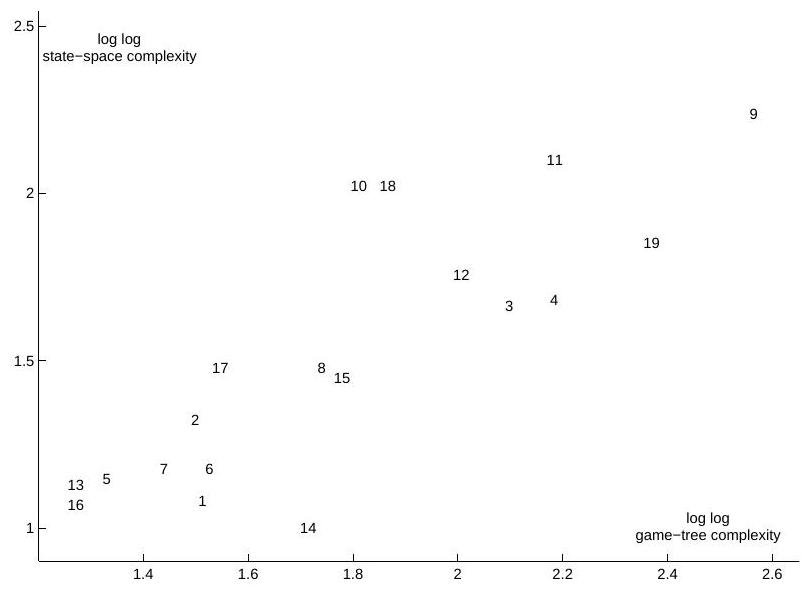
\includegraphics[max width=\textwidth]{2024_09_21_575efd6e0a8f951a52dfg-3}
\end{center}

Figure 4: Approximate positions of games of table 1 in the game space $[7]$

\section*{4 The Havannah Agent}
In order to construct a Havannah playing agent there first has to be a robust architecture which incorporates a fast representation of the game and its rules. Because the methods to determine a winning connection are nontrivial Subsection 4.1 will be devoted to explain these methods. Subsection 4.2 will describe the Monte-Carlo

Tree Search (MCTS) algorithm as described in [2] which is used in the Havannah agent to search for the best move. This subsection will be divided into the different strategies of which this algorithm consists. Finally, Subsection 4.3 will explain an enhancement made to the agent with the purpose of achieving a more realistic simulation.

\subsection*{4.1 Winning Connections}
To keep the representation of the game as fast as possible, it is best to examine only the newly formed connections when a new piece is placed on the board. Therefore whenever a new piece is placed this can only mean three things viz. (1) an isolated piece is placed, (2) an existing connection is extended or (3) two or three existing connections are connected to form a new connection. Only in the last two cases the architecture will test these connections for a winning situation. Now to test for a bridge or a fork on the one hand is straightforward. In the first case it checks whether the connection contains two different corner cells. In the second case it checks whether the connection contains cells of at least three different board sides and whether the connection contains any corner cells which can be omitted so that a winning connection can still be formed. To check if the connection is a ring on the other hand is not straightforward. A ring can be regarded as a connection of stones which all have at least two neighbours. Moreover, if a stone has exactly two neighbours they should not be neighbours of each other. These conditions are the basis for this method. Any stone which does not comply to these conditions is iteratively removed from the connection. If this results in a connection length of at least six, a ring must exist. Figure 5 a shows a side effect of this method which does not affect the outcome. The method does not remove the centre black stone, for it has six neighbours. It regards the complete seven stone connection as a ring. The connection in Figure 5b will not be considered a ring. Starting with removing the leftmost or rightmost stone this connection will be reduced to zero stones. This method of iteratively removing stones from the connection is a lot cheaper with regard to computation time than an expensive cycle path-finding algorithm.

\subsection*{4.2 Monte-Carlo Tree Search}
Because building an adequate evaluation function in Havannah is quite complex, traditional search algorithms applied to the game tree will perform poorly when lacking this function. To bypass this shortcoming MonteCarlo Tree Search is applied which mainly uses the result of an actual game played in self-play as an evaluation function [3]. The more games won in the game tree going through a certain node the more probable it is that this is the best node. To explain how MCTS works it is best

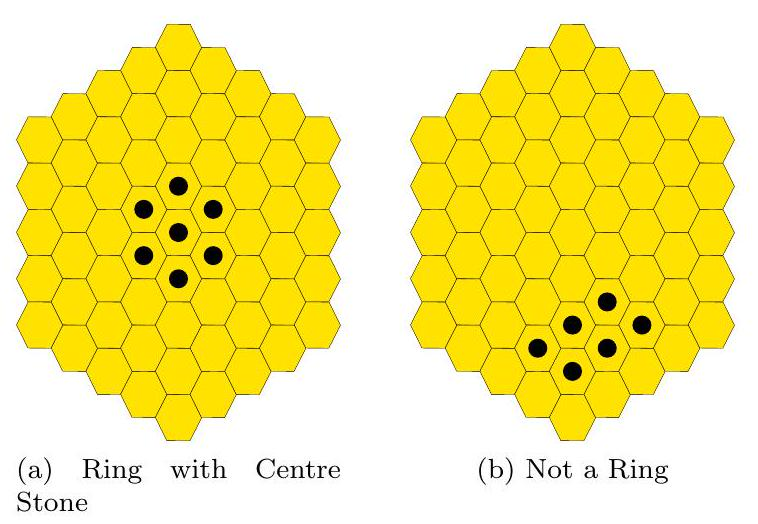
\includegraphics[max width=\textwidth, center]{2024_09_21_575efd6e0a8f951a52dfg-4(1)}\\
Figure 5: Ring and Non-ring Examples\\
to describe it by its four parts outlined in Figure 6. The most important parts are the selection strategy and the simulation strategy. These strategies mainly determine the strength of the MCTS agent.

\begin{center}
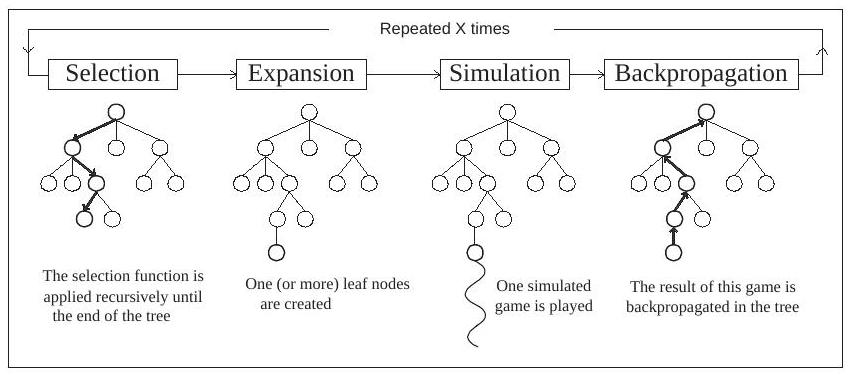
\includegraphics[max width=\textwidth]{2024_09_21_575efd6e0a8f951a52dfg-4}
\end{center}

Figure 6: Outline of a Monte-Carlo Tree Search [2]

\section*{Selection}
Selecting which route to travel down the path of the game tree is an essential part of MCTS. For MCTS to find the optimal move it needs to have a good balance between exploring the search space and exploiting a promising move. When the algorithm tends too much towards exploration, a broad game tree is constructed, which might take too long to converge to the optimal move. When a single path is exploited too fast a suboptimal move might be found which is not the best move overall. This happens when the algorithm is too exploitative. Hence a good strategy has to be found, which uses an optimal balance between these two properties. In this paper the Upper Confidence bound applied to Trees (UCT) [8] is used. UCT is easy to implement and works as follows. Let $I$ be the set of nodes reachable from the current node $p$. UCT selects the child $k$ of node $p$ that satisfies Formula 3 as in [2]:


\begin{equation*}
k \in \arg \max _{i \in I}\left(v_{i}+C \times \sqrt{\frac{\ln n_{p}}{n_{i}}}\right) \tag{3}
\end{equation*}


where $v_{i}$ is the value of the node $i, n_{i}$ is the visit count of $i$ and $n_{p}$ is the visit count of $p$. The constant $C$ determines the balance between exploration and exploitation. This value is tuned experimentally, which will be described in Section 5 and is set to $C=1.2$. Thus when a certain node in the path often leads to success the more likely it is this node will get selected. UCT is usually only applied when a node exceeds a certain visit count threshold. For this research the threshold $T \geq 50$ is used. When the node is below this threshold the simulation strategy determines which node gets selected.

\section*{Expansion}
After the selection strategy has selected an appropriate node which is not already in the game tree this node is created and added to the game tree. Unless this node is a terminal state, the simulation strategy discussed in the next paragraph will simulate the game from here until it reaches the end of the game. This part of the algorithm is called expansion.

\section*{Simulation}
The simulation strategy picks the moves to be played in self-play until the game ends. This strategy is not only applied when a simulated game is played. It is also applied as the selection strategy when a certain node has not exceeded the threshold of required visits. In this paper the main strategy consists of pure random play. This strategy was used to test against a greedy Monte-Carlo agent and to tune the previously mentioned $C$ constant. The next section describes an enhancement or heuristic made to the simulation strategy to make it more realistic. On the one hand these heuristics are necessary to create a strong MCTS agent. On the other hand, if these enhancements or heuristics are too deterministic this can lead to too much exploitation, hence a weaker agent. Moreover, the application of heuristics takes time, this may slow down the simulations. Therefore a good balance has to be found between time spent on heuristics and time spent on simulations.

\section*{Backpropagation}
When the simulated game in self-play has ended, the leaf node and the parent nodes up until the root of this leaf node have to be updated with the result. This procedure is called backpropagation. A game can be a win, a loss or a draw, which propagates $+1,-1$ or 0 , respectively through the nodes backwards.

\section*{Final Move Selection}
The four steps described in the previous paragraphs are one iteration of the MCTS algorithm. These steps are repeated as long as there is time left. As described in [2] a number of ways to select the final move are present. The Havannah MCTS agent selects the node with the highest value. The actual value of a node is calculated as the sum of the results divided by the number of visits through this node.

\subsection*{4.3 Nearest Neighbour Preference}
As mentioned, the main parts of the MCTS algorithm are the selection strategy and the simulation strategy. There are several ways in which enhancements to the method can be made. For instance, when incorporating perfect knowledge into the algorithm, this can prove that certain paths down the tree are wins or losses. This kind of enhancement is not applied in this paper but will be discussed in the final section. For this paper an enhancement to the simulation strategy is made. The basic version of the MCTS agent uses pure random simulations when a node is played out in self-play. This random play hardly resembles any realistic human play. Observing that Havannah is a connection game it would be more logical to focus the simulation near the previously played move or the opponent's previously played move. This leads to the Nearest Neighbour (NN) preference. This heuristic ranks available moves according to their distance to the previously played move. This can either be based solely on the player's own last move, or on both players' last moves. In the last case a coin toss decides whether to focus on the player's own move or the opponent's move. Now moves closest to the last played move have the highest chance to be selected for the next move.

\section*{5 Performance}
In order to discuss the results of the Monte-Carlo Tree Search (MCTS) agent it is necessary to describe the way this agent evolved from simpler agents. These evolving steps are discussed in the next section. On the basis of these steps the experimental setup will become clear. The last section will give a detailed overview of the actual conducted experiments and the outcomes.

\subsection*{5.1 Experimental Setup}
The first step in the creation of a more advanced agent is to create a simple autonomously playing Havannah agent. This is a pure randomly playing agent. Any advancement made to the agent should outperform this agent. The random agent is only capable of making legal moves. The second step was the creation of a simple Monte-Carlo simulation based agent. This agent will serve as the main reference for tuning the MCTS agent. Its strategy is a very greedy one, based merely on its own success. Therefore it will be referenced as the Greedy agent. It uses random play to simulate games for every available position until there is no more time left. The position with the highest score is selected as the move to be played. This opportunistic strategy ignores the opponent's certain winning moves. Nevertheless this simple\\
aggressive play is often hard to parry especially when a frame is created. The lacking of defensive play by the Greedy agent is compensated by the MCTS agent. Implementing the MCTS algorithm is also the final step in the agent's refinement. The strength of this agent is determined by its capability to foresee the creation of a frame or to create a faster one. Although neither the Greedy nor the MCTS agent have formal knowledge of frames or frame threats, creating or detecting them is intrinsic to the Monte-Carlo approach and the underlying mathematical structure of Havannah. The only thing uncertain is how fast it will find them.

The above mentioned three agents viz. Random agent, Greedy agent and MCTS agent, are the basis for the experiments conducted. A number of experiments have been conducted to optimize the strength of the MCTS agent against the Greedy agent. Another number of experiments have been conducted to test an enhancement made to the simulation strategy. These experiments will be outlined in the next subsection.

\subsection*{5.2 Experiments and Results}
The first experiment conducted is to test how well the Greedy agent and the MCTS agent play against the Random agent. The experiments are performed on a $9 \times 9$ and a $19 \times 19$ board by playing 200 games. In every experiment the agent tested plays an equal amount of games as white and black to compensate for the possible advantage of moving first. Both agents get 5 seconds to think about their move. Both the Greedy and the MCTS agent achieve a $100 \%$ win rate on every board.

The second experiment is to optimize the $C$ constant used in Formula 3 as discussed in Section 4. The same conditions of the first experiment apply in this experiment. The only exception is that the $19 \times 19$ board is excluded from the experiments. The $C$ constant is varied from 0.2 to 1.8 in steps of 0.2 . For every constant value 100 games are played. The results are displayed in Table 2. Based on the results the $C$ constant is set to 1.2 in any further experiments.

Table 2: Tuning of MCTS $C$ constant against Greedy agent

\begin{center}
\begin{tabular}{cccccccccc}
\hline
 & \multicolumn{10}{c}{$C$ constant} \\
\cline { 2 - 10 }
 & 0.2 & 0.4 & 0.6 & 0.8 & 1 & 1.2 & 1.4 & 1.6 & 1.8 &  \\
\hline
Average win & 0.41 & 0.55 & 0.7 & 0.66 & 0.66 & 0.76 & 0.71 & 0.68 & 0.69 &  \\
\hline
\end{tabular}
\end{center}

The third series of experiments determines the strength of the Nearest Neighbour (NN) preference enhancement made to the simulation strategy. This is tested by playing 200 games with a Greedy and an MCTS agent with the NN preference against a Greedy and an MCTS agent without the preference. Both with the preference focusing solely on the player's own last move and the coin toss method discussed in Section 4. Both agents again have 5 seconds to think about their move. For reference the results of the Random agent with the NN preference against the one without the preference are also added. These are obtained by simulating 100,000 games. Table 3 shows the results of this experiment. To test whether the enhancement performs

Table 3: Strength of the NN preference on $9 \times 9$

\begin{center}
\begin{tabular}{llrrr}
\hline
 &  & \multicolumn{3}{c}{NN enhancement} \\
\cline { 3 - 5 }
 &  & Random agent & Greedy agent & MCTS agent \\
\hline
\multirow{2}{*}{Average win} & Coin toss & 0.51 & 0.43 & 0.43 \\
 & Own Last Move & 0.51 & 0.46 & 0.48 \\
\hline
\end{tabular}
\end{center}

better on a $19 \times 19$ board, experiments with similar conditions as in the previous series are conducted. Due to fact that the Havannah agent is in infancy and testing it for $19 \times 19$ is time consuming only 100 games for the Greedy and MCTS agent are played. Table 4 reveals the outcome of this experiment.

The results indicate that the Nearest Neighbour preference does not improve the Greedy and MCTS agent's play on $9 \times 9$. On $19 \times 19$ only the Greedy agent seems to perform better when preferring only his own last move. Focusing on the own last move seems to be the best strategy for the Greedy and MCTS agent on any board.

Table 4: Strength of the NN preference on $19 \times 19$

\begin{center}
\begin{tabular}{llrrr}
\hline
 &  & \multicolumn{3}{c}{NN enhancement} \\
\cline { 3 - 5 }
 &  & Random agent & Greedy agent & MCTS agent \\
\hline
\multirow{2}{*}{Average win} & Coin toss & 0.55 & 0.41 & 0.35 \\
 & Own Last Move & 0.55 & 0.55 & 0.47 \\
\hline
\end{tabular}
\end{center}

\section*{6 Conclusions}
With a state-space complexity of $10^{127}$ and a game-tree complexity of $10^{157}$, Havannah is a difficult game to solve. Because evaluating Havannah positions is very difficult traditional Tree Search algorithms are hard to apply. Monte-Carlo simulations are a suited alternative. The Greedy Monte-Carlo agent and the MCTS agent both have a $100 \%$ win rate against the Random agent. Using Monte-Carlo Tree Search with the Upper Confidence bound applied to Trees even shows a $76 \%$ win rate against the Greedy agent. This is a considerable improvement. An idea is to revise the pure random simulation strategy to make the agent more advanced. By introducing the Nearest Neighbour preference the performance of the agent did not improve. With the excep-\\
tion of the Greedy agent with own last move NN preference on $19 \times 19$ the performance of the Monte-Carlo based agents dropped. The coin toss property shows an overall drop of performance.

To summarize the results: given Havannah's complexities and difficulty of developing an evaluation function, MCTS is a well-suited technique for creating a Havannah agent. The pure random character of the simulation remains a huge point of improvement. Applying the Nearest Neighbour preference to the simulation strategy did not have the intended result. The strongest agent developed is the MCTS agent with the pure random simulation strategy. This agent is assumed to be a good opponent for a beginning Havannah player. A more skilled player will exploit the agent's inability to create or prevent a frame and is therefore no match for the MCTS agent.

\section*{7 Future Research}
Future research on and improvements to the Havannah agent should focus on expanding it with knowledge. As discussed in Section 2 frames are the most important strategic goals to pursue. If an agent is capable of detecting frames the MCTS algorithm could be extended with perfect knowledge. This could lead to the agent being able to prove wins or losses in certain paths. The first step in gaining this knowledge is for the agent to have notion of virtual connections, since a frame is a virtual connection. The current idea of keeping track of connections could easily be extended to incorporate virtual connections. Therefore a different representation of the board is needed and a few observations. Figure 7 shows the representation intended, which leads to the following array representation.

\begin{center}
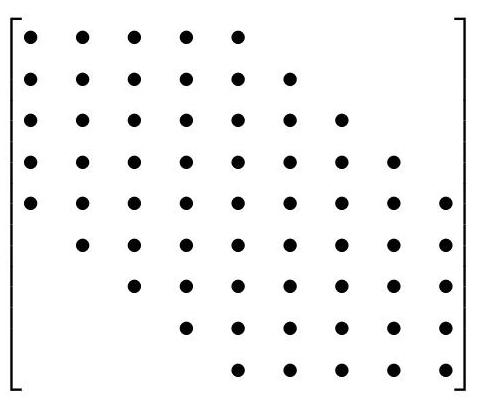
\includegraphics[max width=\textwidth]{2024_09_21_575efd6e0a8f951a52dfg-7}
\end{center}

Here a $\bullet$ means a legal tile. The upper left corner stands for position $(1,1)$. Now observe that a position in the array can have up to eight neighbours, viz. left $(\leftarrow)$, right $(\rightarrow)$, up $(\uparrow)$, down $(\downarrow)$, top-left $(\nwarrow)$, bottom-left $(\swarrow)$, top-right ( $\nearrow$ ), bottom-right ( $($ ). The arrows can be regarded as simple array transformations. Only neighbours $\leftarrow, \rightarrow, \uparrow, \downarrow, \nwarrow$ and $\searrow$ correspond to actual neighbours on the Havannah board. Neighbours $\nearrow$ and $\swarrow$ correspond to 2-bridge connected tiles. A Havannah tile can have up to six 2-bridge connected tiles. Position $(1,1)$ has two 2-bridge connected tiles: $(3,2)$ and $(2,3)$. Some 2-bridge connected tiles can be reached via two routes, for example $\uparrow \nwarrow$ and $\nwarrow \uparrow$ lead to the same tile. For any position in the array, the following transformations are, if legal, 2-bridge connected tiles: $\nearrow, \swarrow,(\uparrow \nwarrow$ or $\nwarrow \uparrow),(\backslash \leftarrow$ or $\leftarrow \nwarrow),(\rightarrow \searrow$ or $\searrow, \rightarrow)$ and $(\searrow \downarrow$ or $\downarrow \searrow)$. These simple array transformations allow for a fast check of 2-bridges. Instead of using a Nearest Neighbour preference in the simulation strategy, a 2-bridge preference could be implemented. This could lead to a more realistic simulation. Detecting 2 -bridges is also essential in evaluating positions. Analogue to keeping track of real connections, placing a stone can mean either three things viz. (1) a new virtual connection of size 1 is created, (2) an existing virtual connection is extended, (3) two virtual connections are connected to form a single virtual connection. Being able to keep track of the virtual connections is the first step in recognizing frame or terminal state threats.

\begin{center}
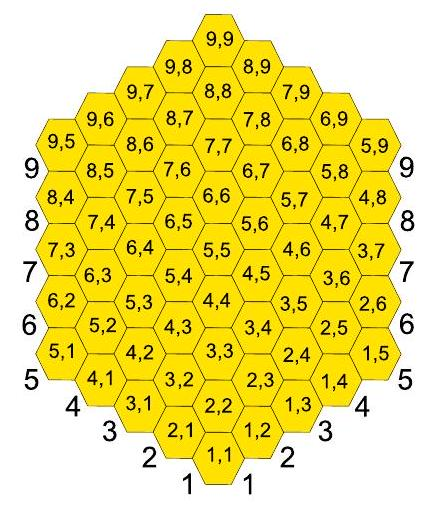
\includegraphics[max width=\textwidth]{2024_09_21_575efd6e0a8f951a52dfg-7(1)}
\end{center}

Figure 7: Alternative board representation

\section*{References}
[1] Allis, L.V. (1994). Searching for Solutions in Games and Artificial Intelligence. Ph.D. thesis, Maastricht University.\\
[2] Chaslot, G.M.J-B., Winands, M.H.M., Herik, H.J. van den, Uiterwijk, J.W.H.M., and Bouzy, B. (2008). Progressive Strategies for Monte-Carlo Tree Search. New Mathematics and Natural Computation, Vol. 4, No. 3, pp. 343-357.\\
[3] Coulom, R. (2007). Efficient Selectivity and Backup Operators in Monte-Carlo Tree Search. Proceedings of the 5th International Conference on Computer and Games (eds. H.J. van den Herik, P. Ciancarini, and H.H.L.M. Donkers), Vol. 4630 of Lecture Notes in Computer Science (LNCS), pp. 72-83, Springer-Verlag, Heidelberg, Germany.\\
[4] Freeling, C. (2003a). Basic Tactics Part 1. Abstract Games, pp. 14-15. Issue 15.\\
[5] Freeling, C. (2003b). Basic Tactics Part 2. Abstract Games, pp. 18-20, 24. Issue 16.\\
[6] Freeling, C. (2003c). Introducing Havannah. Abstract Games, p. 14. Issue 14.\\
[7] Herik, H.J. van den, Uiterwijk, J.W.H.M., and Rijswijck, J. van (2002). Games solved: Now and in the future. Artificial Intelligence, Vol. 134, No. 1-2, pp. 277-311.\\
[8] Kocsis, L. and Szepesvári, C. (2006). Bandit Based Monte-Carlo Planning. Machine Learning: ECML 2006 (eds. J. Fürnkranz, T. Scheffer, and M. Spiliopoulou), Vol. 4212 of Lecture Notes in Artificial Intelligence, pp. 282-293.\\
[9] Marsland, T.A. (1992). Computer Chess and Search. Encyclopedia of Artificial Intelligence (ed. S. Shapiro), pp. 224-241, J. Wiley \& Sons, 2nd edition.\\
[10] Rijswijck, J. van (2000). Are Bees Better Than Fruitflies - Experiments with a Hex Playing Program. Advances in Artificial Intelligence: 13th Biennial Conference of the Canadian Society for Computational Studies of Intelligence, pp. 13-25.\\
[11] Teytaud, F. and Teytaud, O. (2009). Creating an Upper-Confidence-Tree program for Havannah. $A C G 12$ (eds. H.J. van den Herik and P.H.M. Spronck), To appear in Lecture Notes in Computer Science (LNCS), Springer-Verlag, Berlin, Germany.


\end{document}